
\section{Google: Learning Hand-Eye Coordination for Robotic Grasping}

\begin{frame}{\insertsec}
Paper published by Sergey Levine \emph{et al.} (2016).
Its objective is for a robot to learn how to grab pieces by using only image data and a movement
and rotation vector.

\begin{center}
    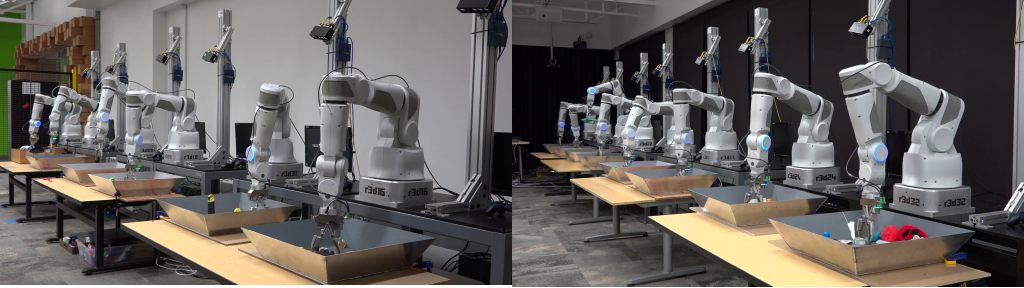
\includegraphics[width=.9\textwidth]{images/google_robot}
\end{center}
\end{frame}


\begin{frame}
Network with both image input and scalar input, each value is repeated 
\(img.width \times img.height\) times to match the CNN size.
\begin{center}
    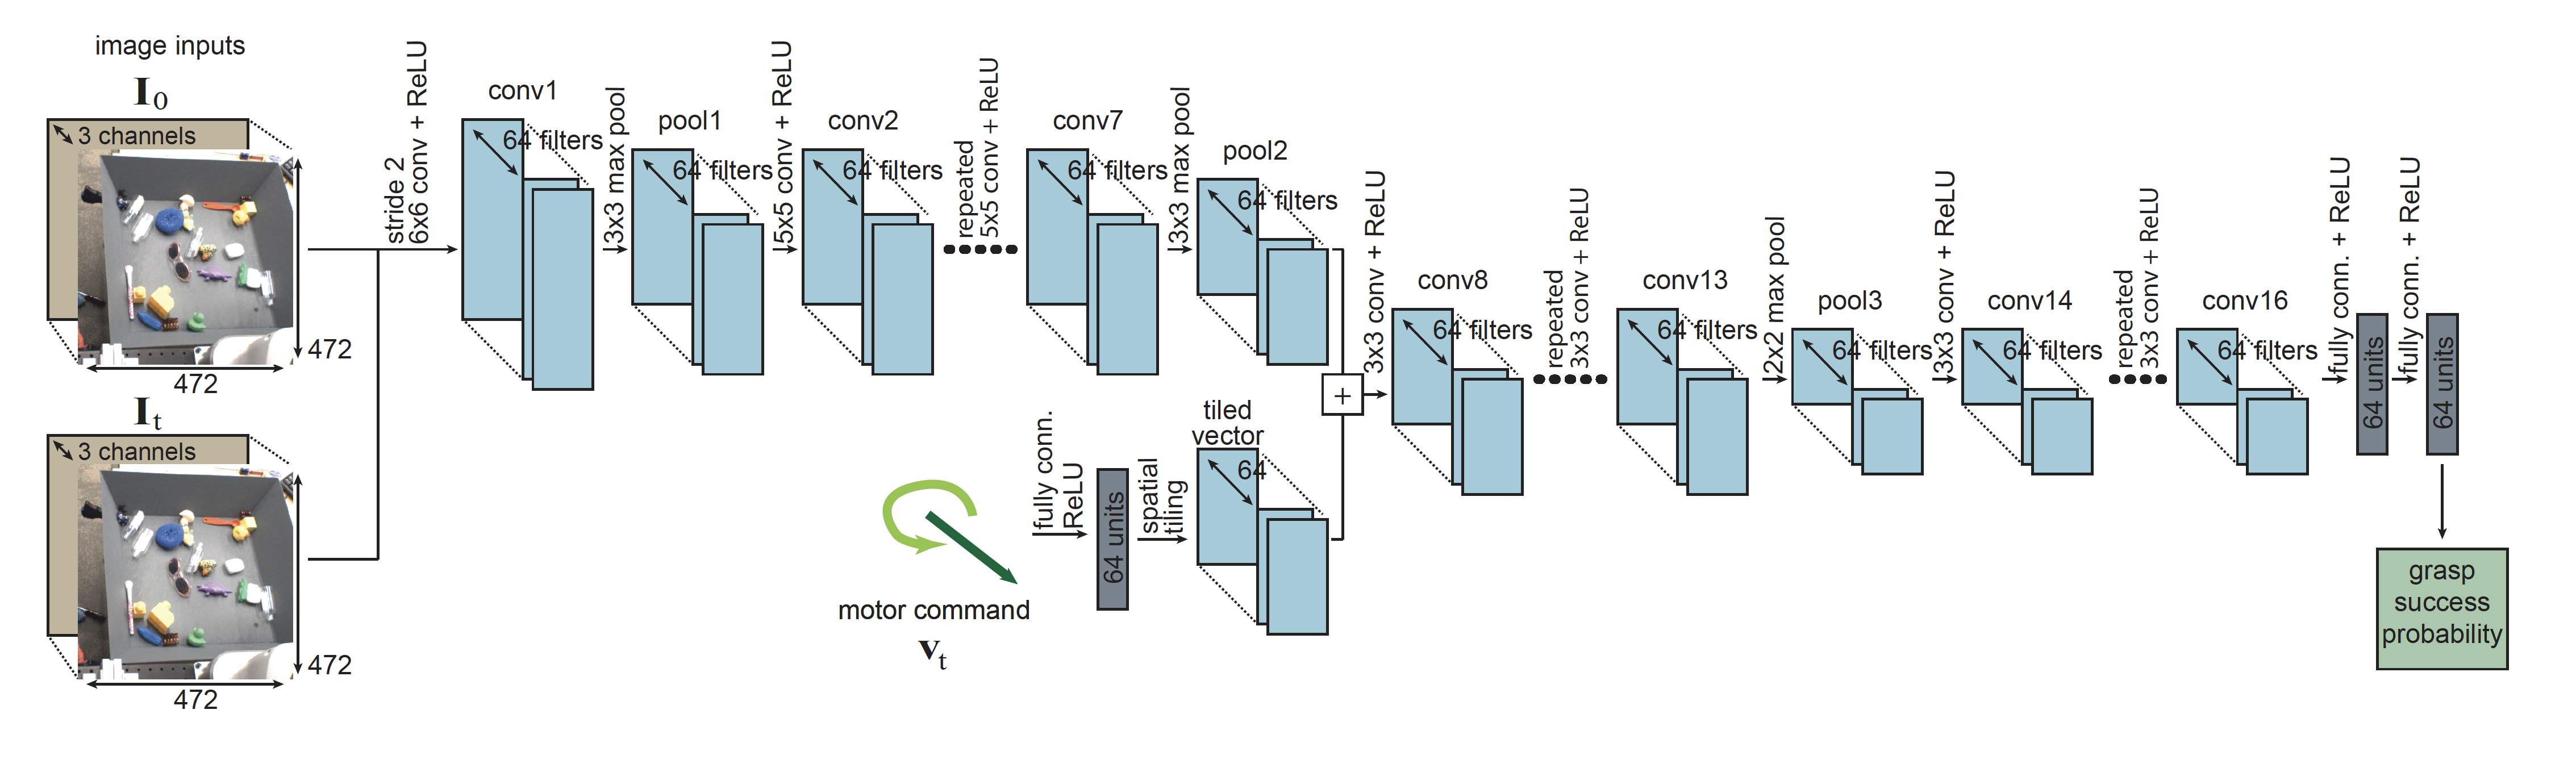
\includegraphics[width=\textwidth]{images/google_robot_network}
\end{center}
\end{frame}